\begin{figure}
    \centering
    \begin{minipage}{0.32\textwidth}
        \centering
        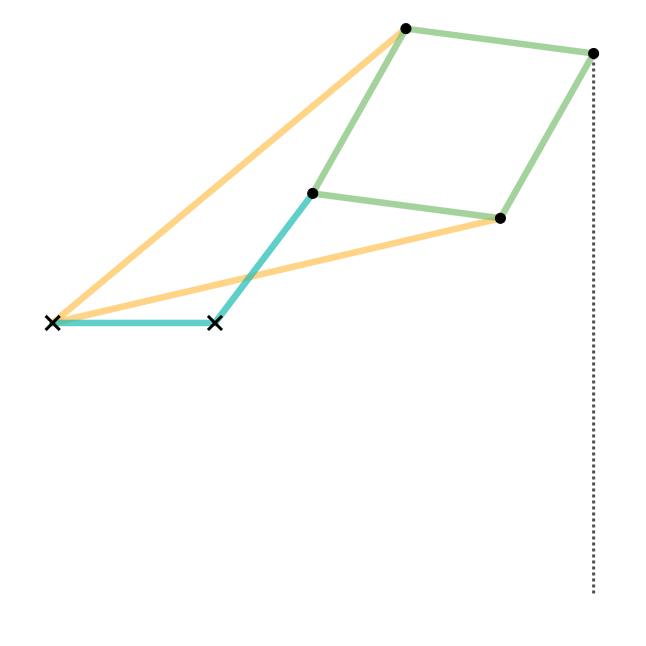
\includegraphics[width=\textwidth]{papers/geradlinig/figures/peaucellier_linkage1.png}
    \end{minipage}
    \hfill
    \begin{minipage}{0.32\textwidth}
        \centering
        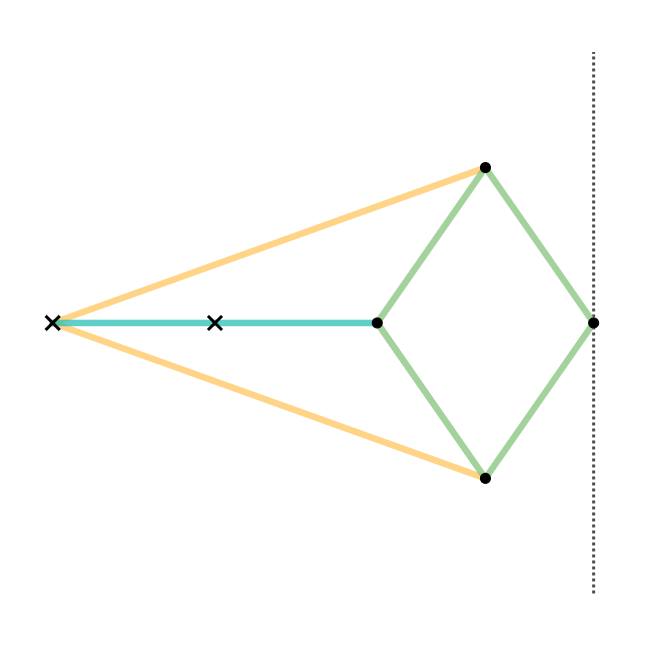
\includegraphics[width=\textwidth]{papers/geradlinig/figures/peaucellier_linkage2.png}
    \end{minipage}
    \hfill
    \begin{minipage}{0.32\textwidth}
        \centering
        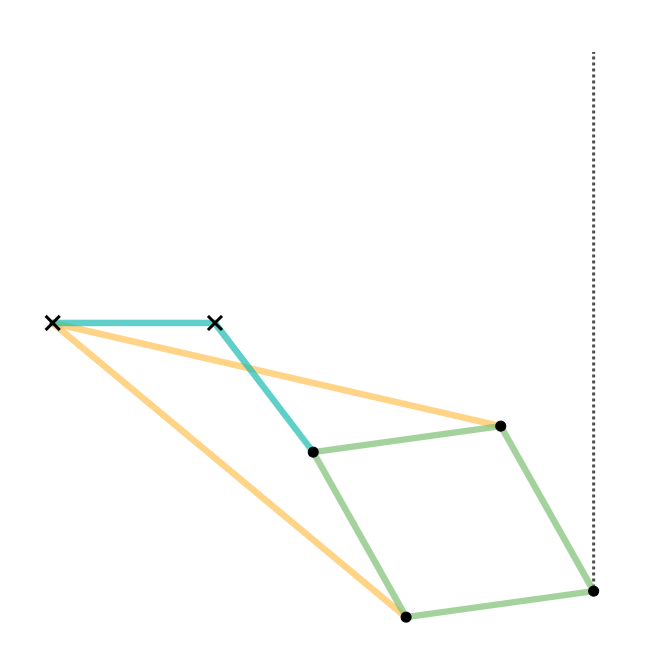
\includegraphics[width=\textwidth]{papers/geradlinig/figures/paucellier_linkage3.png}
    \end{minipage}
    \caption{Der Mechanismus von Peaucellier und Lipkin~\cite{peauc_lip_linkage}.}
    \label{fig:peaucellier_link}
\end{figure}
